\documentclass[10pt]{article}
\usepackage{icmlko}

\icmlmeta{IP 파운데이션 월드모델}{233}{정직한 것만 벌받았다}{노트 232가 하네스 한 줄을 고쳤다. 누가 더 걸렸는지 훑었더니 하나뿐이고, 그 하나가 유일하게 정직한 정식화였다}

\begin{document}

\twocolumn[
\icmlheader

\begin{abstract}
노트 232가 \texttt{rankdata} 의 NaN 전파를 고치고 ``부분 NaN 을 내는 다른
정식화가 있나''를 남겼다. 열여섯을 훑었다. \textbf{하나뿐이다} ---
F1 프로크루스테스가 아홉 도메인 중 여덟에서 부분 NaN 이고
\textbf{2,528 표본(98.6\%)이 사라질 뻔했다.} 나머지 열넷은 전부 9/9
온전이다. \textbf{왜 F1 만인지가 이 노트의 요지다.} 다른 정식화는 축이
없으면 중립 대입 $+$ 관측 표시자로 채운다(노트 85) --- \emph{모든} 행에
숫자를 내므로 NaN 이 안 생긴다. F1 만 완전사례 분해라 못 매기는 행이
남고, \textbf{그것을 정직하게 NaN 으로 돌려준다.} 그래서 \textbf{정직하게
NaN 을 돌려주는 유일한 정식화가 유일하게 벌받았다} --- 대충 채우는 쪽은
아무 벌도 안 받았다. 그리고 노트 231이 ``죽은 정식화 둘''로 센 나머지
하나도 다시 봤다. \textbf{F17 은 고장이 아니라 해당 없음이다} ---
\texttt{grp} 로 시작하는 축만 쓰는데 그 판에는 그 열이 0 개라 빈 자료가
되고 \texttt{axis\_order} 가 빈 사전에서 터진다. \textbf{무리 축이 있는
판에서는 멀쩡하다} --- \texttt{grp} · \texttt{trendcalgrp} 에서 9/9
도메인 · 2,608 표본 · 판 $-$0.2511 이고, \textbf{음수라는 것 자체가
정보다}(무리 축만 쓰면 반대로 맞힌다). 고쳤다 --- \texttt{axis\_order} 가
빈 입력에서 안 터지고, F17 이 해당 없는 판에서 예측을 전부 NaN 으로 돌려
\textbf{덮음 0 으로 드러난다.} 이제 세 상태가 갈린다: \textbf{살아있음}
(9/9) · \textbf{해당 없음}(0/9, 가드가 잡는다) · \textbf{고장}(예외).
전에는 뒤의 둘이 똑같이 크래시로 보였다.
\end{abstract}
]

\begin{figure*}[t]
\centering
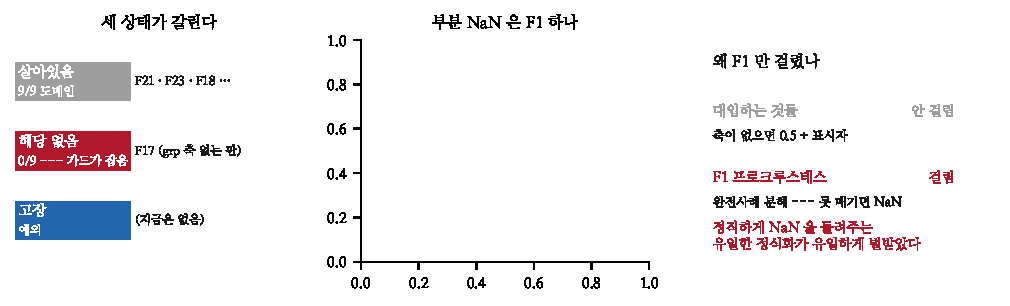
\includegraphics[width=\textwidth]{figs/threestates.pdf}
\caption{왼쪽 --- 세 상태. 가운데 --- 부분 NaN 은 하나뿐. 오른쪽 ---
왜 그 하나인가.}
\end{figure*}

\section{하나뿐이다}

\begin{table}[t]
\centering\tsize
\caption{trendcalwiki 에서 예측의 NaN 무늬(도메인 9개 기준).}
\begin{tabular}{lrrrr}
\toprule
& 온전 & 부분 & 전무 & 잃을 뻔 \\
\midrule
\textbf{F1 프로크루스테스} & 1 & \textbf{8} & 0 & \textbf{2{,}528} \\
F17 무리전용 & 0 & 0 & \textbf{9} & 0 \\
\midrule
F0 · F10$\times$3 · F11$\times$2 & 9 & 0 & 0 & 0 \\
F12 · F16 · F18 · F19 & 9 & 0 & 0 & 0 \\
F21 · F23 & 9 & 0 & 0 & 0 \\
\bottomrule
\end{tabular}
\end{table}

\claimx{\textbf{부분 NaN 을 내는 것은 F1 하나다.} 그 하나가 유보 2,565
중 \textbf{2,528(98.6\%)} 을 잃을 뻔했다 --- 고치기 전에는 실제로
잃었다.}{나머지 열넷은 전부 9/9 온전이다. \textbf{버그가 포트폴리오
전체를 위협한 것이 아니라 정확히 한 항목을 겨눴다} --- 그리고 그 항목이
기준선이었다.}

\section{정직한 것만 벌받았다}

\claimx{\textbf{다른 정식화는 축이 없으면 중립 대입 $+$ 관측 표시자로
채운다}(노트 85) --- \emph{모든} 행에 숫자를 내므로 NaN 이 안
생긴다.}{\textbf{F1 만 완전사례 분해라 못 매기는 행이 남고, 그것을
정직하게 NaN 으로 돌려준다.} 그래서 \textbf{정직하게 NaN 을 돌려주는
유일한 정식화가 유일하게 벌받았다} --- 대충 채우는 쪽은 아무 벌도 안
받았다.}

\claimx{\textbf{이것이 하네스가 만드는 선택압이다.} ``모르는 것을
모른다고 말하는'' 정식화가 판정치에서 지워지면, 남는 것은 모르는 것도
채우는 정식화뿐이다.}{노트 85가 중립 대입을 도입할 때 ``축이 없는
도메인도 채점하려면 채워야 한다''고 적었다 --- \textbf{맞는 결정이었지만
그 결정이 대안을 벌한다는 것은 안 적었다.}}

\section{고장이 아니라 해당 없음}

\begin{table}[t]
\centering\tsize
\caption{F17 무리전용.}
\begin{tabular}{lrrrl}
\toprule
축 판 & grp 열 & 판 & 도메인 & \\
\midrule
grp & 10 & $-$.2511 & 9/9 & 정상 \\
trendcalgrp & 10 & $-$.2511 & 9/9 & 정상 \\
\textbf{trendcalwiki} & \textbf{0} & --- & \textbf{0/9} & \textbf{해당 없음} \\
\bottomrule
\end{tabular}
\end{table}

\claimx{\textbf{F17 은 고장이 아니다} --- \texttt{grp} 축이 있는 판에서는
9/9 도메인 · 2,608 표본으로 멀쩡하다. \textbf{판이 $-$0.2511 인 것 자체가
정보다}(무리 축만 쓰면 반대로 맞힌다).}{\texttt{grp} 열이 0 인 판에서
빈 자료가 되고 \texttt{axis\_order} 가 빈 사전에서 터졌다 ---
\textbf{노트 231이 ``죽은 정식화 둘''로 센 것이 하나는 틀렸다.}}

\claimx{\textbf{세 상태를 가른다} --- 살아있음(9/9) · 해당 없음(0/9,
가드가 잡는다) · 고장(예외). \textbf{전에는 뒤의 둘이 똑같이 크래시로
보였다.}}{고침은 둘이다: \texttt{axis\_order} 가 빈 입력에서 안 터지고,
F17 이 해당 없는 판에서 예측을 전부 NaN 으로 돌려 덮음 0 으로 드러난다.}

\begin{table}[t]
\centering\tsize
\caption{이 훑기가 안 본 것.}
\begin{tabular}{ll}
\toprule
F2 결합 잠재 & 적합 1회 110초 --- 뺐다 \\
F18 · F6 의 recent 변형 & 느려서 뺐다 \\
\bottomrule
\end{tabular}
\end{table}

\claimx{\textbf{이 훑기 자체의 덮음을 적는다} --- 열여섯 중 셋을 안 봤다
(F2 결합 잠재, F18 · F6 의 recent 변형). 시간 때문이다.}{\textbf{덮음을
적는 노트가 자기 덮음을 안 적으면 안 된다.} 안 본 셋은 다 대입하는
계열이라 부분 NaN 이 안 날 것으로 보지만 \emph{그것은 짐작이다} ---
노트 232에서 짐작을 세 번 틀렸다.}

\begin{table}[t]
\centering\tsize
\caption{남은 것.}
\begin{tabular}{ll}
\toprule
\textbf{안 본 셋} & F2 · recent 둘 --- 마저 훑을 것 \\
\textbf{선택압} & 대입이 벌 안 받는 것이 옳은가 \\
F1 복귀 & 기준선이 $+$0.2447 로 돌아왔다 \\
\bottomrule
\end{tabular}
\end{table}

둘째 줄이 이 세 노트(231$\sim$233)가 실제로 연 물음이다. \textbf{하네스가
``모르는 것을 모른다''고 말하는 정식화를 벌하면, 포트폴리오는 대입하는
쪽으로만 자란다.} 지금 열여섯 중 열다섯이 대입 계열이고 하나가 완전사례
계열인데, \textbf{그 하나가 백 노트 동안 죽어 있었다는 것이 그 선택압의
증거다.} 노트 85의 중립 대입은 맞는 결정이었지만, \textbf{대입한 것과
관측한 것을 판정치가 구분하지 않는 한 ``채우면 이긴다''가 성립한다} ---
그것을 재는 것이 다음이다.

\end{document}
